


The Peierls model is based on a linear elastic formulation of the energy, perhaps with a fitted misalignment potential. Other formulations might provide more insight. Empirical potentials have been developed for a wide range of materials and conditions for the field of molecular dynamics. These potentials are computationally tractable, at least compared to quantum mechanical treatments, while hopefully retaining enough fidelity to actual behaviour to give physical insight \cite{martinez2013}.

Various potentials exist for different types of materials, which usually are applicable to only some classes of materials. For example, the embedded atom method applies well to metals \cite{Daw1984}, the Lennard-Jones and Buckingham potentials describe dispersion interactions, and the short range exchange interaction arising from Pauli exclusion \cite{Jones1924,Buckingham1938} and bond order potentials describe covalent bonding, e.g. the Tersoff potential \cite{Tersoff1988}. 


Ionic solids are an ideal class of materials with which to demonstrate the application of alternative energy calculations by applying empirical potentials. Some modelling of dislocation motion by the conventional Peierls-Nabarro model, using the elastic properties and the generalised staking fault energy, has been undertaken for \ce{MgO} \cite{Miranda2005}, however the chemical bonding is well described by fairly simple empirical potentials that could provide more insight into the factors controlling plasticity than linear elasticity. 

There are large numbers of ionic solids with the same simple crystal structures, e.g. rock salt and caesium chloride \cite{Kelly2012app7}, and the primary contribution to the energy of these materials is the electrostatic interaction, which is mathematically simple:
\begin{equation}
U^{\text{electro}}_{ij} = \frac{1}{4\pi\epsilon_0} \frac{q_i q_j}{r_{ij}}
\end{equation}
where $\epsilon_0$ is the permittivity of free space, $q_i$ is the charge on atom $i$ and $r_{ij}$ is the separation between atoms $i$ and $j$.


The Lennard-Jones potential is often used to capture the shorter range interaction in ionic solids. The Lennard-Jones is one of the simplest formulations to represent these interactions in ionic solids and has the form:
\begin{equation}
\phi_{ij}(r_{ij}) = 4\epsilon_{ij} \left[ \left( \frac{\sigma_{ij}}{r_{ij}}\right)^{12}-     \left( \frac{\sigma_{ij}}{r_{ij}}\right)^6   \right]
\end{equation}
or in the ``A--B'' form:
\begin{equation}
\phi_{ij}(r_{ij}) = \frac{A_{ij}}{r_{ij}^{12}} - \frac{B_{ij}}{r_{ij}^{6}}
\end{equation}
where $r_{ij}$ is the atomic separation, $\epsilon_{ij}$ is the depth of the energy minimum, $\sigma_{ij}$ is the atomic separation at which the energy is zero and $A_{ij}$ and $B_{ij}$ are simply parameters to be fitted and are related to $\epsilon_{ij}$ and $\sigma_{ij}$ by $A_{ij} = 4\epsilon_{ij}\sigma_{ij}^{12}$ and $B_{ij} = 4 \epsilon_{ij} \sigma_{ij}^{6}$. The total energy for a pair of atoms is then:
\begin{equation}
U_{ij}(r_{ij}) = \frac{1}{4\pi\epsilon_0} \frac{q_i q_j}{r_{ij}} + \frac{A_{ij}}{r_{ij}^{12}} - \frac{B_{ij}}{r_{ij}^{6}}
\end{equation}




The energy of perfect ionic crystals is relatively easily calculated  via a Madelung or Ewald summation \cite{madelung1918,Ewald1921}, but these usually rely on an assumption of symmetry; an assumption that is broken by the introduction of a defect. In the case of a dislocated crystal another approach is required. One option is a direct sum, which scales with the square of the number of atoms in the simulation. If the distance from the dislocation line is considered the simulation time scales with the fourth power, which can rapidly become intractable. However advances in computing hardware and efficient implementations of array operations in NumPy \cite{Numpy2011}, particularly an efficient implementation of the Einstein summation convention \cite{opt_einsum} may make this a workable solution.


An alternative is to use an implementation of a long range electrostatics solver that allows for non periodicity in two dimensions. One such implementation is the multiscale summation method in LAMMPS \cite{Hardy2009,Plimpton1995,LAMMPS_web}, which divides the problem into one short range potential plus a series of smoothly vanishing long range potentials over increasingly coarse meshes at larger interatomic distances. The use of LAMMPS allows the extension of the energy calculations to other energy terms such as polarisability of ions and so on.


\subsection{Dislocations in ionic crystals}




The rocksalt structure is particularly common in ionic solids and phases of this structure have been widely studied in terms of their plasticity. The slip direction is usually <1\,1\,0> and the active slip planes are \{0\,0\,1\} and \{1\,\={1}\,0\}, and sometimes \{1\,\={1}\,1\}. For edge dislocations the last would expose charged surfaces of atoms at free surfaces, so despite being the closest packed plane it is not commonly seen \cite{Haasen1985}. Schematic illustrations of edge dislocations are shown in \autoref{fig:Schematic_NaCl_dislocs}.

\begin{figure}
\centering
    \begin{subfigure}{0.8\textwidth}
    \centering
    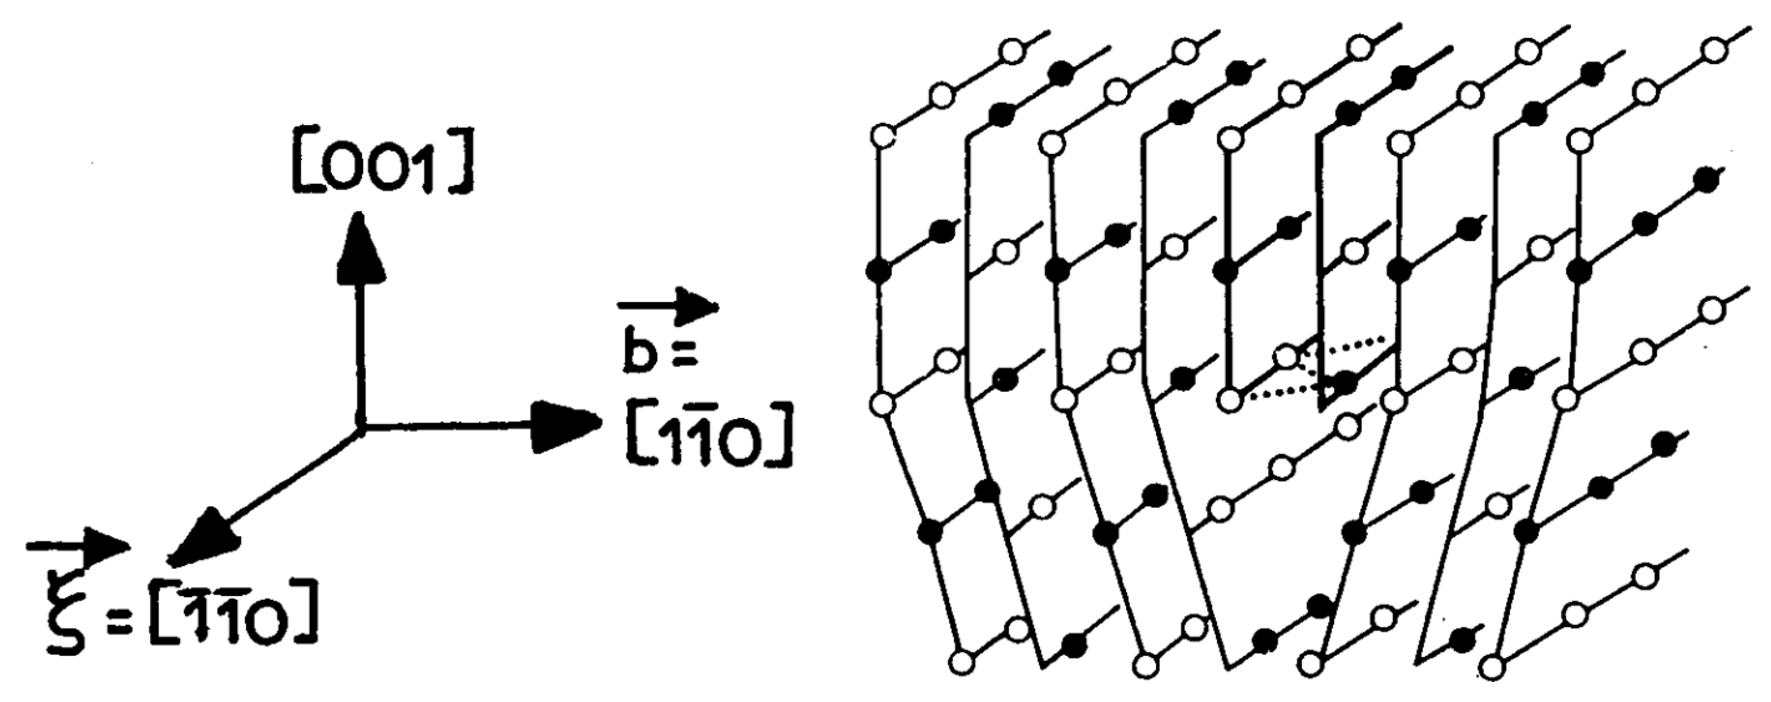
\includegraphics[width=\textwidth]{NaCl_001_1-10}
    \caption{The \{0\,0\,1\}<1\,\={1}\,0> slip system.\label{fig:NaCl_110_001_core_structure}}
    \end{subfigure}
\par\bigskip
    \begin{subfigure}{0.8\textwidth}
    \centering
    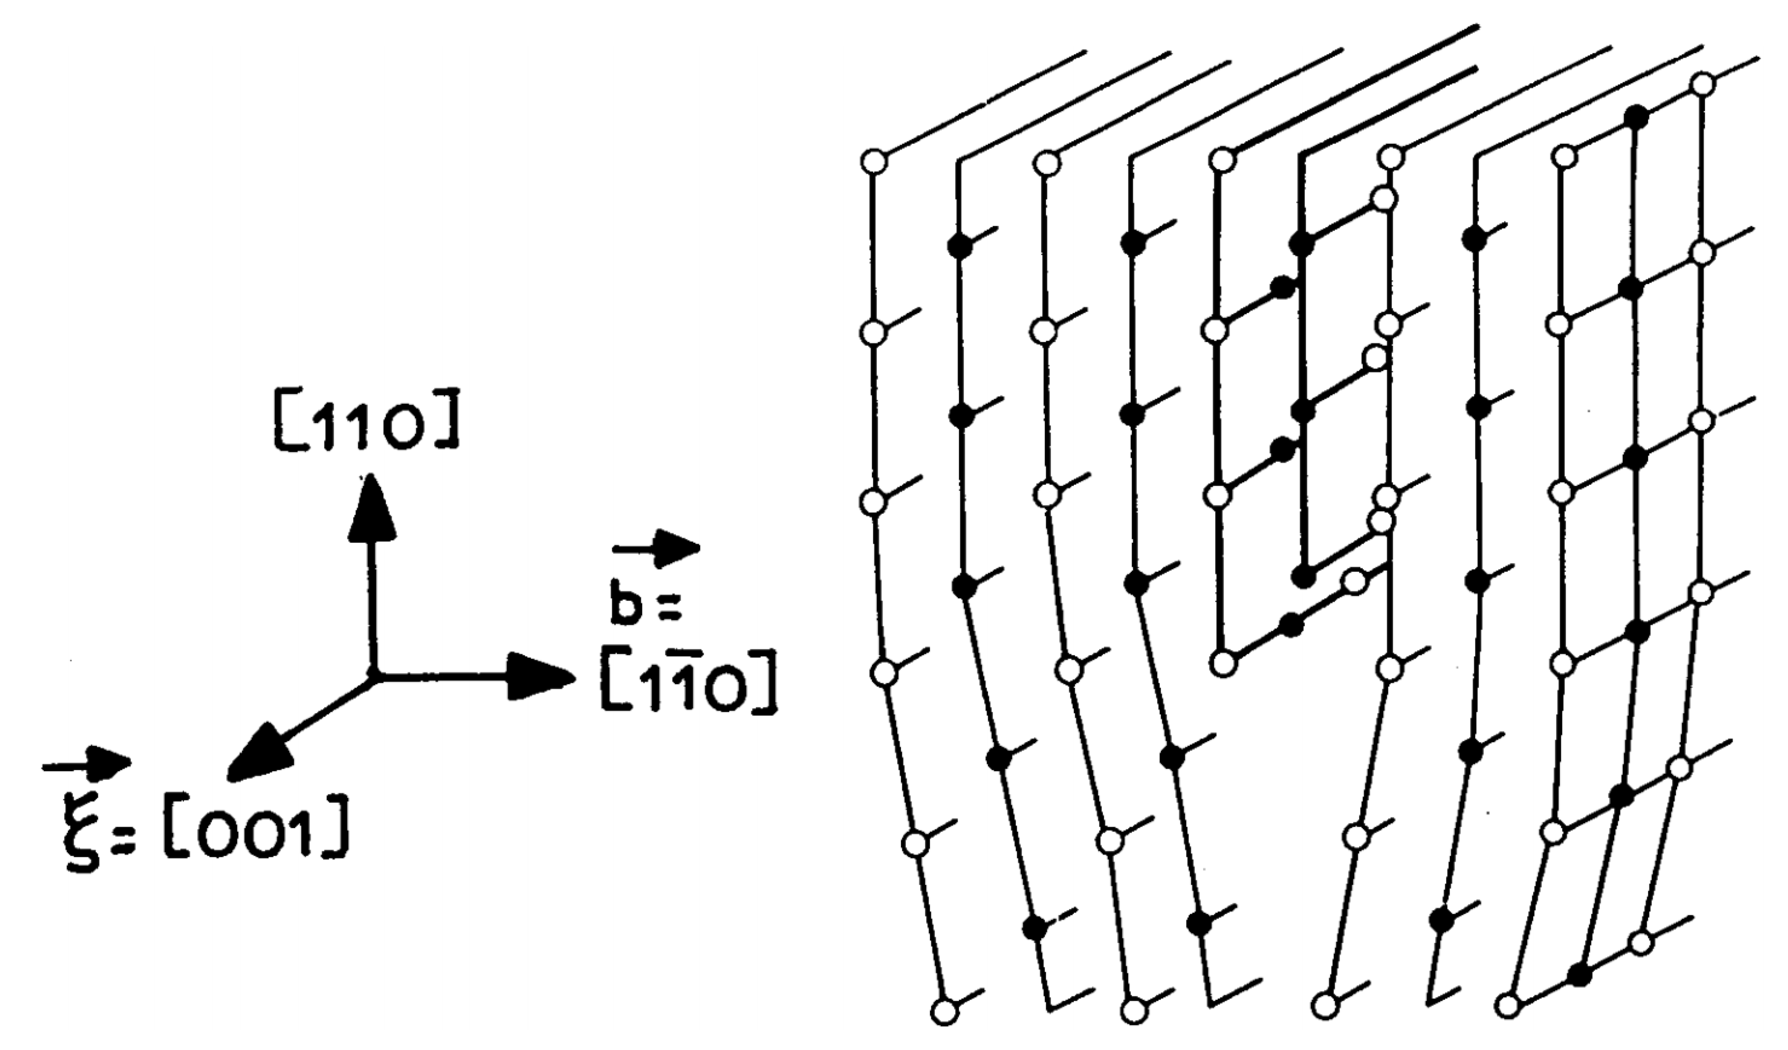
\includegraphics[width=\textwidth]{NaCl_110_1-10}
    \caption{The \{1\,1\,0\}<1\,\={1}\,0> slip system.\label{fig:NaCl_110_110_core_structure}}
    \end{subfigure}
\caption[Edge dislocations in the rock salt crystals.]{Schematic edge dislocations in the rocksalt structure reproduced from \cite{Haasen1985}. \label{fig:Schematic_NaCl_dislocs}}
\end{figure}





Experimental work has characterised the yield stress of ionic solids with the rocksalt structure over a wide range of temperatures, including very low temperatures by using liquid helium (\SI{\sim4}{\kelvin}), and they deviate strongly from the prediction of elastic Peierls models. This makes them useful as a model system for testing dislocation theories \cite{Haasen1985}.

Previous modelling of dislocations in ionic crystals has been undertaken, notably by \citet{puls1976} who simulated edge \{0\,0\,1\}<1\,\={1}\,0> dislocations in \ce{MgO}, and by \citet{Woo1977} who modelled the same dislocation geometry in a range of ionic crystals with the rocksalt structure, among others \cite{Granzer1968,Woo1976,Hoagland1976,Brandt1987,Soullard1991,Foitzik1991}. These were limited by the computational resources available and used a variety of strategies to overcome these limits; one approach was to optimise only the equilibrium position and then assume linear trajectories for the atoms for intermediate states, as developed by \citet{Granzer1968}. This is similar to the assumption made by Peierls \cite{Peierls1940} that the dislocation width does not vary between the equilibrium positions, which has been shown to have a very large effect on the results \cite{Clegg2006,Bulatov1997}.

Another method to overcome computational limitations was to simulate only small regions atomistically. This was achieved by applying a variety of boundary conditions, usually derived from elasticity theory, to constrain the atomistic region and modelling material outside this core region as elastic. Such conditions were used in \cite{Woo1977}. The use of conditions like these prevents the separation of the different energetic components since there is always a large contribution from the elastic region as well as the electrostatics and short-range interactions. A fully atomistic simulation would hopefully show the individual energy contributions and give some insight into the dominant factors  controlling dislocation motion.

A fully atomistic model using suitable interatomic potentials will hopefully illustrate the factors that control dislocation motion in ionic solids.


\section{Summary of background information}


Dislocations are key to the properties of many crystals. In materials such as ceramics and intermetallics the crystal structure itself presents the largest barrier to dislocation motion. This normally limits the applications of ceramic and intermetallic phases which have attractive properties but exhibit such limited plasticity that they are too brittle for structural applications.

There are some ceramic and intermetallic phases, such as the MAX phases or \ce{Nb2Co7}, that do show relatively easy plastic flow, though usually limited to a small number of slip planes. Since this happens in phases with similar chemistry to other, brittle, phases (such as the MAX phases vs TiC and \ce{Nb2Co7} vs \ce{NbCo2}) this change in behaviour is likely to be due to the crystal structure.

The Peierls stress, i.e.\ the lattice resistance in the absence of thermal activation, can be predicted using a Peierls model. There are various such models in the literature that make various assumptions about the nature of the energy calculations and the atomic displacements around the core. The best models make use of the generalised stacking fault, whereby a planar defect is modelled accurately by density functional theory and the results of that model are assumed to be applicable as a misalignment potential in a more element-based model of the dislocation core. Another common assumption is that the atomic displacements are only parallel to the slip plane.

More complex or computationally intractable approaches have gradually been introduced but few, if any, Peierls models have attempted to combine more complex displacement fields and generalised stacking fault energies with an atomistic-scale model of the whole dislocation structure. 

This leads the current work down two distinct, complementary paths. One challenge is to develop the Peierls model to reduce the number of assumptions about atomic positions and the interactions between them. This seems particularly tractable by incorporating complex displacement fields and new energy calculation methods. 

In particular the assumptions that the atomic displacements are only parallel to the slip plane and are small in planes not immediately adjacent to the slip plane and therefore discarded are possible to address by the use of more generalised displacement fields. Such a displacement field then allows the treatment of materials using empirical potentials that apply over long distances, such as the Lennard-Jones potential for ionic materials, potentially addressing the slip in alkali halides that has not been well described by Peierls models based on linear elasticity.

If successful this would open the way to treating the effects of crystal structure on dislocation behaviour more fully. However in the case of a new model the ideal test case is not a complex crystal with behaviour that is not well understood. 

Rather, a model is better developed and tested against well understood behaviour of simpler materials and then applied to complex crystals. For the purposes of developing a model simpler crystals are appropriate, such as pure elements, such as copper, iron and diamond, and simpler covalently bonded crystals such as titanium carbide. This covers a wide range of lattice geometries and yield stresses and is generally well described by exiting models. In this way it can be hoped to improve the generality of the Peierls model and broaden its applicability while also characterising its ability to predict, accurately, known behaviour.

In parallel, there is immediate interest in the low flow stresses observed experimentally in layered crystals such as the MAX phases. This can be addressed by adapting existing methods; using insight into the crystal structure to inform quantum mechanical modelling of complex phases, and altering an existing Peierls model to take account of this.


                      






















